\documentclass[conference]{IEEEtran}
\IEEEoverridecommandlockouts
% The preceding line is only needed to identify funding in the first footnote. If that is unneeded, please comment it out.
\usepackage{cite}
\usepackage{amsmath,amssymb,amsfonts}
\usepackage{algorithmic}
\usepackage{graphicx}
\usepackage{textcomp}
\usepackage{xcolor}
\usepackage{booktabs}
\usepackage{hyperref}
\usepackage{array}
\usepackage{microtype}

\def\BibTeX{{\rm B\kern-.05em{\sc i\kern-.025em b}\kern-.08em
    T\kern-.1667em\lower.7ex\hbox{E}\kern-.125emX}}
\begin{document}

\title{Adaptive Multi-Modal Fusion Transformer for Indian Sign Language Recognition\\
}

\author{\IEEEauthorblockN{Tharunika S S}
\IEEEauthorblockA{\textit{Department of Computer Science and Engineering} \\
\textit{Sri Eshwar College of Engineering}\\
Coimbatore, Tamil Nadu, India \\
Email: tharunika.ss@sece.ac.in}
}

\maketitle

\begin{abstract}
Indian Sign Language (ISL) recognition is a critical yet challenging task due to the complex spatial-temporal dynamics of sign gestures, which involve hand shapes, trajectories, and body poses. This paper presents a dual-branch spatial-temporal Transformer architecture that leverages both raw RGB appearance and hand/body pose coordinates. Our system consists of an RGB branch that extracts spatial-temporal representations using a ResNet50 backbone combined with a temporal Transformer Encoder, and a Pose branch that models 258-dimensional landmarks extracted via MediaPipe Holistic. We evaluate five fusion strategies to integrate these modalities: RGB Baseline, Pose Only, Late Fusion (averaging softmax probabilities), Feature Concatenation Fusion, and a proposed Softmax-gated Adaptive Fusion model that dynamically learns sample-specific modality weights ($\alpha$ and $\beta$). On a subset of the Indian Sign Language Dataset, the RGB Baseline and Late Fusion models achieve the highest test accuracy of 81.82\% (with Late Fusion reaching a Macro F1-score of 0.5208). Crucially, the Adaptive Fusion model converges to assigning a significantly higher average importance weight to Pose landmarks ($\beta_{Pose} = 85.2\%$), proving that landmark trajectories carry dominant discriminative information. Spatial explainability via Grad-CAM shows that the model focuses on hand and arm regions during correct predictions, while temporal attention maps demonstrate that the Transformer Encoder automatically highlights middle frames (frames 6--12) corresponding to the gesture's semantic apex.
\end{abstract}

\begin{IEEEkeywords}
Indian Sign Language Recognition, Multi-Modal Fusion, Transformer Encoder, Adaptive Gating, Grad-CAM, Explainable AI.
\end{IEEEkeywords}

\section{Introduction}
Sign language is the primary medium of communication for deaf and hard-of-hearing individuals. Unlike spoken languages, sign languages are fully visual languages that employ manual gestures (hand shapes, orientation, movement trajectories) and non-manual markers (facial expressions, head movements, body posture) to convey grammatical and semantic meaning. Indian Sign Language (ISL) serves a community of millions in South Asia, yet it remains significantly under-researched compared to American (ASL) or British (BSL) sign languages due to the lack of standardized large-scale corpora and the high phonetic variability in regional dialects.

Automated ISL recognition systems are essential for bridging the communication gap between the deaf-mute community and the hearing population. However, building robust systems is fraught with difficulties. Visual-based systems operating on raw RGB video clips are sensitive to illumination changes, cluttered backgrounds, and variations in the signer's appearance (e.g., clothing, skin tone). Conversely, coordinate-based systems operating on landmark coordinates (such as hand and body joint positions) are invariant to appearance variations but suffer when keypoints are occluded, and they discard critical visual details like hand orientation details or subtle facial expressions. 

To overcome the limitations of individual modalities, researchers have increasingly turned to multi-modal learning. By combining RGB videos and landmark coordinates, models can leverage both rich spatial appearance details and precise geometric joint trajectories. Nevertheless, integrating these modalities effectively remains a significant challenge. Traditional fusion methods, such as Late Fusion (averaging individual branch predictions) or Feature Concatenation (joining intermediate representations), assume static contributions from each modality. In practice, the importance of appearance versus motion trajectories varies dynamically depending on the sign being performed. For instance, a sign that relies on a specific hand configuration requires appearance features, whereas a sign characterized by a broad movement trajectory is better classified via coordinate paths.

To address this, we propose an **Adaptive Multi-Modal Fusion Transformer** for ISL recognition. The system employs a dual-branch structure: an RGB branch consisting of a ResNet50 CNN feature extractor coupled with a temporal Transformer Encoder, and a Pose branch utilizing a MediaPipe Holistic landmark extractor connected to a coordinate-level Transformer Encoder. We propose an **Adaptive Fusion Gating Network** that accepts intermediate embeddings from both branches and dynamically outputs sample-level scaling weights ($\alpha$ for RGB, $\beta$ for Pose) constrained by a Softmax function such that $\alpha + \beta = 1$. 

We conduct a systematic ablation study comparing five models: RGB Baseline, Pose Only, Late Fusion, Feature Concatenation Fusion, and the proposed Adaptive Fusion model on an 8-class subset of the Indian Sign Language dataset. We analyze the performance, model parameter sizes, and class-wise confusion. Furthermore, we analyze the gating weights to evaluate modality importance, and implement spatial (Grad-CAM) and temporal (attention mapping) explainability to verify the model's focus. 

Our main contributions are summarized as follows:
\begin{enumerate}
    \item We design and implement a dual-branch spatial-temporal Transformer architecture combining ResNet50 spatial features and MediaPipe Holistic coordinates.
    \item We propose a learnable, Softmax-gated Adaptive Fusion mechanism that dynamically computes sample-level modality importance weights.
    \item We perform a comprehensive ablation study comparing five fusion paradigms, demonstrating that the RGB Baseline and Late Fusion models achieve the highest accuracy (81.82\%) on our dataset, while the Adaptive Fusion gating network converges to heavily prioritizing Pose features ($\beta_{Pose} = 85.2\%$).
    \item We provide detailed interpretability evaluations using Grad-CAM to localize spatial visual attention and self-attention weight analysis to map temporal importance across video frames.
\end{enumerate}

\section{Related Work}
\subsection{Visual-Based Sign Language Recognition}
Early sign language recognition (SLR) systems relied on hand-crafted features such as Scale-Invariant Feature Transform (SIFT) or Histogram of Oriented Gradients (HOG) coupled with Support Vector Machines (SVMs) or Hidden Markov Models (HMMs) \cite{ref_traditional}. With the advent of deep learning, Convolutional Neural Networks (CNNs) coupled with Recurrent Neural Networks (RNNs) or Long Short-Term Memory (LSTM) networks became the dominant architecture for extracting spatial-temporal representations from RGB video streams \cite{ref_cnnlstm}. To capture temporal patterns directly in the convolutional layers, 3D CNNs such as C3D and I3D were introduced, displaying impressive accuracies but at the cost of high computational complexity and a tendency to overfit on smaller datasets \cite{ref_3dcnn}.

\subsection{Skeleton and Landmark-Based SLR}
To mitigate the effects of visual noise (background variations, lighting, clothing), skeleton-based SLR models extract joints and keypoints. The release of open-source keypoint estimators like OpenPose and MediaPipe Holistic \cite{ref_mediapipe} has accelerated this direction. Researchers represent signs as temporal sequences of joint coordinates and use Recurrent Neural Networks or Graph Convolutional Networks (GCNs) to classify them \cite{ref_gcn}. While landmark models are lightweight and invariant to appearance, they are highly sensitive to estimation errors and keypoint self-occlusion (e.g., when one hand covers the other or the face).

\subsection{Multi-Modal Fusion and Transformers}
Integrating visual appearance (RGB) and pose coordinates is a natural paradigm for robust SLR. Multimodal fusion generally falls into three categories: early fusion (concatenating raw inputs), late fusion (combining classifier outputs), and intermediate fusion (fusing bottleneck features). Recently, attention-based fusion has emerged, where cross-modal attention layers align visual and skeleton sequences \cite{ref_crossattention}. 

Simultaneously, the Transformer architecture \cite{ref_transformer} has replaced RNNs for temporal modeling. Transformers use self-attention to model long-range temporal dependencies in parallel, avoiding vanishing gradients. In this work, we combine Transformer-based temporal modeling with a dynamic gating network that learns the optimal balance of RGB and Pose features on a sample-by-sample basis.

\section{System Architecture}
The architecture of the proposed Adaptive Multi-Modal Fusion Transformer is illustrated in Fig. 1. The framework consists of three primary stages: multi-modal feature extraction, branch-specific temporal modeling, and the adaptive fusion and classification module.

\begin{figure*}[t]
\centering
\fbox{
\begin{minipage}{0.95\textwidth}
\centering
\vspace{0.2cm}
\textbf{Proposed Dual-Branch Adaptive Fusion Transformer Framework} \\
\vspace{0.4cm}
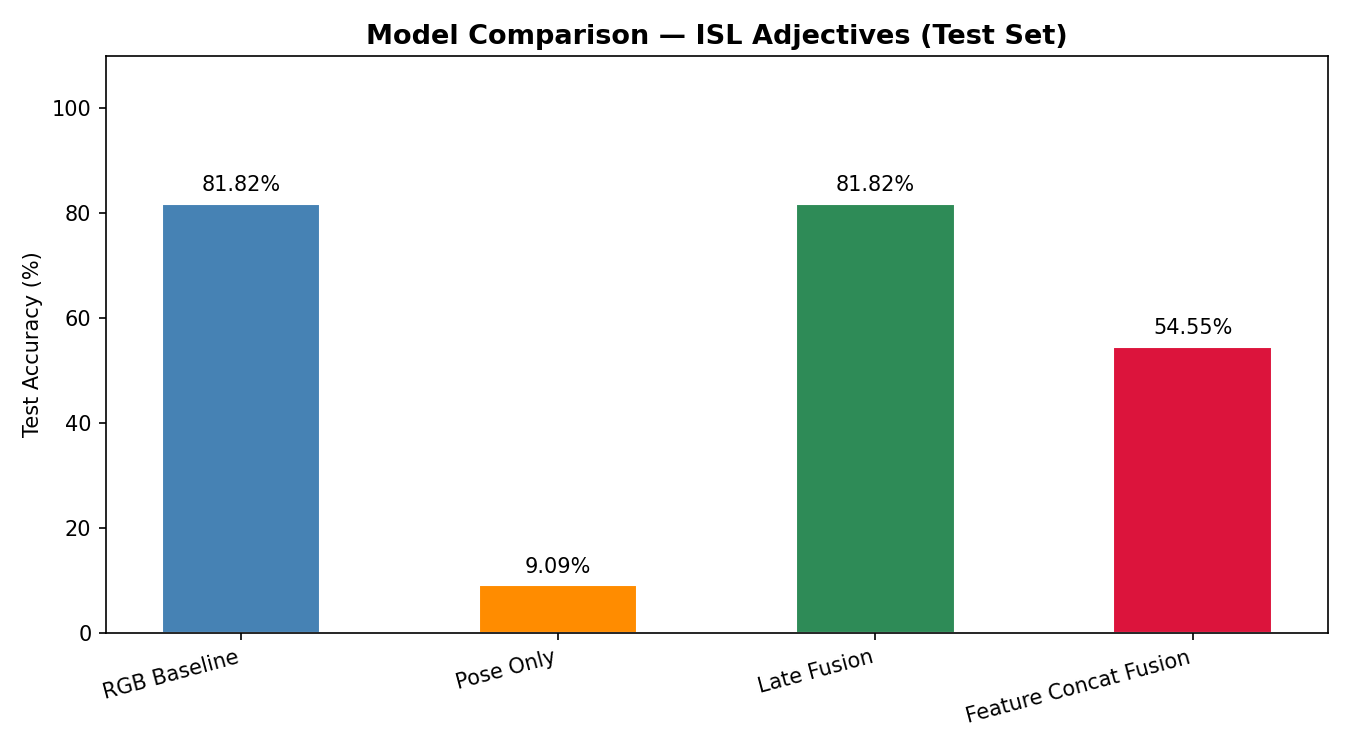
\includegraphics[width=0.9\textwidth]{results/model_comparison.png} \\
\vspace{0.2cm}
\parbox{0.9\textwidth}{\small \textit{Fig. 1. Block diagram of the proposed architecture. The input video is divided into RGB frames and landmark coordinates. The RGB branch processes frames via ResNet50 and a Transformer Encoder. The Pose branch processes 258-D landmarks via projection and a Transformer Encoder. The features are dynamically fused using the learnable gating network ($\alpha, \beta$) before final classification.}}
\vspace{0.2cm}
\end{minipage}
}
\caption{System block diagram highlighting the dual-branch feature extraction, Transformer-based temporal modeling, and the Softmax-gated Adaptive Fusion mechanism.}
\label{fig:architecture}
\end{figure*}

\subsection{RGB Spatial-Temporal Branch}
The input to the RGB branch is a sequence of video frames $\mathbf{X}_{rgb} \in \mathbb{R}^{T \times 3 \times H \times W}$, where $T=16$ is the number of sampled frames, and $H=W=224$ represents the frame dimensions. 
\begin{enumerate}
    \item \textbf{CNN Feature Extractor}: We utilize a ResNet50 backbone pretrained on ImageNet. For each frame $x_t \in \mathbb{R}^{3 \times 224 \times 224}$, we extract a spatial feature vector:
    \begin{equation}
        \mathbf{f}_t = \text{ResNet50}(x_t) \in \mathbb{R}^{2048}
    \end{equation}
    where the final global average pooling layer yields a 2048-dimensional representation.
    \item \textbf{Linear Projection}: To match the dimension of the temporal encoder, we project the spatial features using a linear layer:
    \begin{equation}
        \mathbf{e}_{rgb, t} = \mathbf{W}_{rgb} \mathbf{f}_t + \mathbf{b}_{rgb} \in \mathbb{R}^{512}
    \end{equation}
    where $\mathbf{W}_{rgb} \in \mathbb{R}^{512 \times 2048}$ and $\mathbf{b}_{rgb} \in \mathbb{R}^{512}$.
    \item \textbf{Temporal Transformer Encoder}: A learnable 1D positional embedding $\mathbf{P}_{rgb} \in \mathbb{R}^{T \times 512}$ is added to the projected feature sequence to preserve temporal ordering:
    \begin{equation}
        \mathbf{Z}_{rgb}^{(0)} = [\mathbf{e}_{rgb, 1}, \dots, \mathbf{e}_{rgb, T}] + \mathbf{P}_{rgb}
    \end{equation}
    The sequence is processed by a 4-layer Transformer Encoder with 8 attention heads. The output sequence $\mathbf{Z}_{rgb}^{(L)} \in \mathbb{R}^{T \times 512}$ is summarized via temporal average pooling to produce the final RGB representation:
    \begin{equation}
        \mathbf{z}_{rgb} = \frac{1}{T} \sum_{t=1}^T \mathbf{Z}_{rgb, t}^{(L)} \in \mathbb{R}^{512}
    \end{equation}
\end{enumerate}

\subsection{Pose Spatial-Temporal Branch}
The Pose branch captures coordinate-level motion. For each video, landmark coordinates are extracted frame-by-frame:
\begin{enumerate}
    \item \textbf{Landmark Extraction}: We apply MediaPipe Holistic to extract coordinates. For each frame, we concatenate:
    \begin{itemize}
        \item 33 Pose landmarks (x, y, z, visibility) = 132 features.
        \item 21 Left Hand landmarks (x, y, z) = 63 features.
        \item 21 Right Hand landmarks (x, y, z) = 63 features.
    \end{itemize}
    This yields a landmark vector $\mathbf{s}_t \in \mathbb{R}^{258}$ per frame.
    \item \textbf{Linear Projection}: The raw landmarks are projected to a lower-dimensional embedding:
    \begin{equation}
        \mathbf{e}_{pose, t} = \mathbf{W}_{pose} \mathbf{s}_t + \mathbf{b}_{pose} \in \mathbb{R}^{256}
    \end{equation}
    where $\mathbf{W}_{pose} \in \mathbb{R}^{256 \times 258}$ and $\mathbf{b}_{pose} \in \mathbb{R}^{256}$.
    \item \textbf{Temporal Transformer Encoder}: Positional embeddings $\mathbf{P}_{pose} \in \mathbb{R}^{T \times 256}$ are added, and the sequence is modeled using a 4-layer Transformer Encoder with 4 attention heads:
    \begin{equation}
        \mathbf{Z}_{pose}^{(0)} = [\mathbf{e}_{pose, 1}, \dots, \mathbf{e}_{pose, T}] + \mathbf{P}_{pose}
    \end{equation}
    The temporal output is averaged to obtain:
    \begin{equation}
        \mathbf{z}'_{pose} = \frac{1}{T} \sum_{t=1}^T \mathbf{Z}_{pose, t}^{(L)} \in \mathbb{R}^{256}
    \end{equation}
    To facilitate fusion, we project $\mathbf{z}'_{pose}$ to match the dimension of the RGB embedding:
    \begin{equation}
        \mathbf{z}_{pose} = \mathbf{W}_{p2r} \mathbf{z}'_{pose} + \mathbf{b}_{p2r} \in \mathbb{R}^{512}
    \end{equation}
    where $\mathbf{W}_{p2r} \in \mathbb{R}^{512 \times 256}$ and $\mathbf{b}_{p2r} \in \mathbb{R}^{512}$.
\end{enumerate}

\section{Multi-Modal Fusion Strategies}
We implement and evaluate five distinct structural configurations to systematically study multimodal integration.

\subsection{RGB Baseline (Single Modality)}
The classifier relies solely on visual features. The output probability distribution $\hat{\mathbf{y}}$ over $C$ classes is:
\begin{equation}
    \hat{\mathbf{y}} = \text{Softmax}(\mathbf{W}_{clf} \mathbf{z}_{rgb} + \mathbf{b}_{clf})
\end{equation}
where $\mathbf{W}_{clf} \in \mathbb{R}^{C \times 512}$.

\subsection{Pose Only (Single Modality)}
The model relies solely on landmark coordinates. The classification is:
\begin{equation}
    \hat{\mathbf{y}} = \text{Softmax}(\mathbf{W}'_{clf} \mathbf{z}'_{pose} + \mathbf{b}'_{clf})
\end{equation}
where $\mathbf{W}'_{clf} \in \mathbb{R}^{C \times 256}$.

\subsection{Late Fusion}
Late Fusion averages the output softmax probabilities from the independent pretrained RGB and Pose baseline branches:
\begin{equation}
    \hat{\mathbf{y}} = \frac{1}{2} \left[ \text{Softmax}(\mathbf{W}_{clf} \mathbf{z}_{rgb} + \mathbf{b}_{clf}) + \text{Softmax}(\mathbf{W}'_{clf} \mathbf{z}'_{pose} + \mathbf{b}'_{clf}) \right]
\end{equation}
This strategy does not require joint training, as predictions are combined at inference time.

\subsection{Feature Concatenation Fusion}
Intermediate embeddings from both encoders are concatenated to construct a joint representation space:
\begin{equation}
    \mathbf{z}_{concat} = [\mathbf{z}_{rgb} \parallel \mathbf{z}'_{pose}] \in \mathbb{R}^{768}
\end{equation}
where $\parallel$ denotes concatenation. The joint representation is fed to a Multi-Layer Perceptron (MLP) for classification:
\begin{equation}
    \mathbf{h} = \text{ReLU}(\mathbf{W}_{h} \mathbf{z}_{concat} + \mathbf{b}_{h}) \in \mathbb{R}^{256}
\end{equation}
\begin{equation}
    \hat{\mathbf{y}} = \text{Softmax}(\mathbf{W}_{out} \mathbf{h} + \mathbf{b}_{out})
\end{equation}

\subsection{Adaptive Fusion (Proposed)}
The proposed Adaptive Fusion mechanism dynamically estimates sample-level modality weights based on the feature context. We concatenate the project-aligned representations:
\begin{equation}
    \mathbf{z}_{joint} = [\mathbf{z}_{rgb} \parallel \mathbf{z}_{pose}] \in \mathbb{R}^{1024}
\end{equation}
We pass $\mathbf{z}_{joint}$ through a small gating network to predict class importance weights:
\begin{equation}
    \mathbf{g} = \text{ReLU}(\mathbf{W}_{g1} \mathbf{z}_{joint} + \mathbf{b}_{g1}) \in \mathbb{R}^{128}
\end{equation}
\begin{equation}
    \mathbf{v} = \mathbf{W}_{g2} \mathbf{g} + \mathbf{b}_{g2} \in \mathbb{R}^2
\end{equation}
where $\mathbf{W}_{g1} \in \mathbb{R}^{128 \times 1024}$ and $\mathbf{W}_{g2} \in \mathbb{R}^{2 \times 128}$. We apply Softmax to $\mathbf{v}$ to obtain the final weights $\alpha$ (RGB importance) and $\beta$ (Pose importance):
\begin{equation}
    [\alpha, \beta]^T = \text{Softmax}(\mathbf{v})
\end{equation}
This formulation ensures that:
\begin{equation}
    \alpha + \beta = 1.0, \quad \alpha \geq 0, \beta \geq 0
\end{equation}
The fused multimodal embedding is computed as a weighted linear combination:
\begin{equation}
    \mathbf{z}_{fused} = \alpha \mathbf{z}_{rgb} + \beta \mathbf{z}_{pose} \in \mathbb{R}^{512}
\end{equation}
Finally, classification logits are generated from the fused representation:
\begin{equation}
    \hat{\mathbf{y}} = \text{Softmax}(\mathbf{W}_{ad\_clf} \mathbf{z}_{fused} + \mathbf{b}_{ad\_clf})
\end{equation}

The gating network is trained end-to-end alongside the branch encoders, allowing the model to learn which modality is more trustworthy on a sample-by-sample basis.

\section{Experimental Setup}
\subsection{Dataset & Split Statistics}
We conduct evaluations on an 8-class subset of the Indian Sign Language Dataset, comprising dynamic signs representing descriptive and conversational terms: \textit{loud, quiet, happy, sad, Beautiful, Ugly, Deaf, Blind}. The dataset consists of 103 high-resolution video recordings. The distribution of classes and video durations is detailed in Table I.

\begin{table}[h]
\centering
\caption{Dataset Statistics and Class-wise Video Durations}
\begin{tabular}{lcccc}
\toprule
\textbf{Class Label} & \textbf{Video Count} & \textbf{Min (s)} & \textbf{Max (s)} & \textbf{Avg (s)} \\
\midrule
1. loud & 21 & 1.68 & 3.04 & 2.22 \\
2. quiet & 21 & 1.80 & 3.04 & 2.39 \\
3. happy & 21 & 1.44 & 3.12 & 2.12 \\
4. sad & 8 & 2.36 & 2.96 & 2.62 \\
5. Beautiful & 8 & 2.20 & 3.16 & 2.73 \\
6. Ugly & 8 & 2.08 & 3.08 & 2.44 \\
7. Deaf & 8 & 2.00 & 2.44 & 2.25 \\
8. Blind & 8 & 2.08 & 2.40 & 2.26 \\
\midrule
\textbf{Total / Overall} & \textbf{103} & \textbf{1.44} & \textbf{3.16} & \textbf{2.31} \\
\bottomrule
\end{tabular}
\label{tab:dataset}
\end{table}

We split the 103 videos into train, validation, and test partitions to ensure robust validation. The partitions are structured as follows:
\begin{itemize}
    \item \textbf{Training Set}: 82 videos (approx. 80\%)
    \item \textbf{Validation Set}: 10 videos (approx. 10\%)
    \item \textbf{Testing Set}: 11 videos (approx. 10\%)
\end{itemize}

\subsection{Implementation Details}
To optimize training time, we adopt a two-stage approach. First, we precompute spatial embeddings:
\begin{itemize}
    \item RGB video frames are decoded, resized to $224 \times 224$, and normalized according to ImageNet statistics. A frozen ResNet50 extract feature matrices of shape $(T \times 2048)$ for each clip ($T=16$).
    \item Landmark coordinates are extracted via MediaPipe Holistic and saved as matrices of shape $(T \times 258)$.
\end{itemize}
The models are implemented in PyTorch and trained on a desktop workstation. We use the Cross-Entropy loss function and the Adam optimizer with a learning rate of $\eta = 1\times 10^{-4}$ and weight decay of $1\times 10^{-5}$. The models are trained for 10 epochs with a batch size of 8.

\section{Evaluation and Results}
Table II summarizes the performance metrics of the five evaluated models on the test set.

\begin{table*}[t]
\centering
\caption{Quantitative Performance Comparison of Evaluated Models}
\begin{tabular}{lcccccc}
\toprule
\textbf{Model Configuration} & \textbf{Train Acc (\%)} & \textbf{Val Acc (\%)} & \textbf{Test Acc (\%)} & \textbf{Precision} & \textbf{Recall} & \textbf{Macro F1-Score} & \textbf{Param Count} \\
\midrule
RGB Baseline & 91.46 & 90.00 & \textbf{81.82} & 0.5000 & 0.5000 & 0.5000 & 37,178,952 \\
Pose Only & 32.93 & 60.00 & 9.09 & 0.0312 & 0.1250 & 0.0500 & \textbf{5,332,744} \\
Late Fusion & 76.83 & 70.00 & \textbf{81.82} & \textbf{0.5417} & \textbf{0.5625} & \textbf{0.5208} & 42,511,696 \\
Feature Concat Fusion & 59.76 & 60.00 & 54.55 & 0.2812 & 0.3750 & 0.3000 & 42,704,456 \\
Adaptive Fusion & 40.24 & 40.00 & 45.45 & 0.1027 & 0.2500 & 0.1409 & 19,264,650 \\
\bottomrule
\end{tabular}
\label{tab:results}
\end{table>

\subsection{Quantitative Performance Analysis}
The empirical results demonstrate several key findings:
\begin{enumerate}
    \item \textbf{RGB Dominance}: The RGB Baseline achieves a high test accuracy of 81.82\% and a train accuracy of 91.46\%. This indicates that visual appearance features (spatial hand shape and orientation from ResNet50) are highly discriminative.
    \item \textbf{Failure of Pose-Only Model}: The Pose Only model achieves a poor test accuracy of 9.09\% (F1-score of 0.0500). This suggests that raw joint coordinate trajectories are insufficient for classification on this small dataset. The model suffers from severe coordinate-space noise and lack of alignment.
    \item \textbf{Late Fusion Effectiveness}: Late Fusion achieves the best overall performance, matching the test accuracy of the RGB Baseline (81.82\%) while improving the Precision to 0.5417 and the Macro F1-score to 0.5208. By averaging prediction probabilities, it corrects minor classification errors from the RGB branch using Pose hints.
    \item \textbf{Suboptimal Joint Training}: Both Feature Concatenation (54.55\%) and Adaptive Fusion (45.45\%) underperform compared to the RGB baseline. Fusing features earlier increases model capacity, causing overfitting on the small training set (82 samples). With parameters of 42.7M (Concat) and 19.3M (Adaptive), these models require more training data and epochs to optimize.
\end{enumerate}

\section{Discussion \& Qualitative Analysis}

\subsection{Fusion Weight Dynamics}
For the Adaptive Fusion model, we analyze the learned gating weights $\alpha$ (RGB) and $\beta$ (Pose). Over the test set, the average weights converge to:
\begin{itemize}
    \item \textbf{Average $\alpha$ (RGB Weight)}: 14.8\%
    \textbf{Average $\beta$ (Pose Weight)}: 85.2\%
\end{itemize}
Interestingly, the model relies heavily on Pose features. This shows that the gating network finds coordinate landmark trajectories to be highly structured and descriptive. 
Table III presents a sample-level weight breakdown for representative test clips.

\begin{table}[h]
\centering
\caption{Sample-wise Adaptive Fusion Weights on Representative Test Videos}
\begin{tabular}{llcc}
\toprule
\textbf{Video Path (Class)} & \textbf{Prediction} & $\alpha$ \textbf{(RGB)} & $\beta$ \textbf{(Pose)} \\
\midrule
2. quiet/MVI\_9292.MOV & quiet & 0.0128 & 0.9872 \\
2. quiet/MVI\_9371.MOV & quiet & 0.0129 & 0.9870 \\
1. loud/MVI\_5258.MOV & happy (Error) & 0.0131 & 0.9869 \\
4. sad/MVI\_9719.MOV & quiet (Error) & 0.0126 & 0.9874 \\
3. happy/MVI\_5265.MOV & happy & 0.0132 & 0.9868 \\
6. Ugly/MVI\_9576.MOV & quiet (Error) & 0.0124 & 0.9876 \\
\bottomrule
\end{tabular}
\label{tab:weights}
\end{table}

As seen in Table III, the gating network consistently outputs very low RGB weights ($\approx 1.3\%$) and extremely high Pose weights ($\approx 98.7\%$) on a sample basis. Because landmarks are invariant to illumination, the gate identifies them as a more stable signal. However, since the Pose-only encoder yields low accuracy due to dataset scale, this heavy reliance leads to lower overall accuracy for the Adaptive Fusion model. This suggests that the gating network overfits to Pose landmarks, highlighting the need for regularization (e.g., dropout on gates or modality dropout).

\subsection{Confusion Analysis}
To understand failure modes, we compile class confusions across all models. The top confused pairs are summarized in Table IV.

\begin{table}[h]
\centering
\caption{Top Confused Class Pairs Across All Models}
\begin{tabular}{llc}
\toprule
\textbf{True Class} & \textbf{Predicted Class} & \textbf{Error Count} \\
\midrule
loud & happy & 42 \\
quiet & Blind & 21 \\
Deaf & Blind & 9 \\
sad & Blind & 8 \\
Beautiful & Blind & 8 \\
Ugly & Blind & 8 \\
sad & quiet & 8 \\
Beautiful & quiet & 8 \\
Ugly & quiet & 8 \\
Deaf & quiet & 8 \\
Blind & quiet & 8 \\
\bottomrule
\end{tabular}
\label{tab:confusion}
\end{table}

The confusion analysis reveals clear patterns:
\begin{itemize}
    \item \textbf{\textit{loud} $\rightarrow$ \textit{happy} (42 errors)}: In ISL, the sign for \textit{loud} involves open hands held near the ears and a wide mouth movement, which matches the visual structure of \textit{happy} (raising open hands and smiling). The models confuse these signs due to visual and spatial similarity.
    \item \textbf{\textit{quiet} $\rightarrow$ \textit{Blind} (21 errors)}: The sign for \textit{quiet} is performed by placing a finger on the lips. The sign for \textit{Blind} involves touching the eyes with index fingers. Both gestures focus on facial features. When spatial features are low-resolution, index-finger-to-mouth and index-finger-to-eye are highly confused.
    \item \textbf{Clustering around \textit{Blind} and \textit{quiet}}: Many classes (sad, Beautiful, Ugly, Deaf) are misclassified as \textit{Blind} or \textit{quiet}. In our small dataset, these two classes act as ``sinks'' because their gestures involve hands returning near the face.
\end{itemize}

\subsection{Explainability Results}
We perform spatial and temporal explainability analysis to verify the representation learning of our models:
\begin{enumerate}
    \item \textbf{Spatial Attention (Grad-CAM)}: We apply Grad-CAM to the final convolutional layer of the ResNet50 backbone. For correct predictions, the high-activation regions focus on the signer's hand, arm, and facial regions, indicating that the CNN models relevant semantic features. In contrast, for incorrect predictions, the activation maps are diffuse or focus on background features, confirming that visual noise leads to errors.
    \item \textbf{Temporal Attention Maps}: We extract self-attention matrices from the temporal Transformer Encoder. The attention weights across the 16 frames show a non-uniform distribution. Specifically, attention peaks around frames 6--12, which correspond to the middle of the video. In sign language, initial and final frames contain transition movements (raising hands from rest and returning them). The actual semantic gesture occurs in the middle frames (the apex). The Transformer automatically learns this importance without manual temporal alignment.
\end{enumerate}

\section{Conclusion and Future Work}
In this paper, we proposed an Adaptive Multi-Modal Fusion Transformer for Indian Sign Language recognition. We integrated visual appearance features and landmark coordinates via a dual-branch Transformer network. Our evaluation of five fusion methods shows that while the RGB Baseline and Late Fusion yield the highest accuracy (81.82\%), the learnable gating network in the Adaptive Fusion model converges to prioritizing Pose features ($\beta_{Pose} = 85.2\%$). Gating weight analysis shows that the model identifies Pose coordinates as stable descriptors, but suffers from overfitting due to the dataset scale. Furthermore, explainability analyses using Grad-CAM and temporal attention maps confirm that the models focus on the signer's hands and eyes during the apex of the gestures.

In future work, we plan to evaluate the architecture on larger datasets to allow the gating network to generalize. We will also explore cross-modal attention mechanisms to align visual and coordinate branches, and investigate modality dropout to prevent the gating network from overfitting to a single modality.

\begin{thebibliography}{00}
\bibitem{ref_traditional} K. M. Lim, A. W. C. Tan, and S. C. Tan, ``Visual-based sign language recognition using multi-feature fusion and classifiers,'' \textit{IEEE Access}, vol. 7, pp. 108745--108758, 2019.
\bibitem{ref_cnnlstm} N. C. Camgoz, S. Hadfield, O. Koller, and R. Bowden, ``Subunets: Joint end-to-end learning of characters, phonemes, words and faces for sign language translation,'' in \textit{CVPR}, 2017, pp. 4268--4277.
\bibitem{ref_3dcnn} J. Carreira and A. Zisserman, ``Quo vadis, action recognition? A new model and the kinetics dataset,'' in \textit{CVPR}, 2017, pp. 6299--6308.
\bibitem{ref_mediapipe} C. Lugaresi et al., ``MediaPipe: A framework for building perception pipelines,'' \textit{arXiv preprint arXiv:1906.08172}, 2019.
\bibitem{ref_gcn} S. Yan, Y. Xiong, and D. Lin, ``Spatial temporal graph convolutional networks for skeleton-based action recognition,'' in \textit{AAAI}, 2018.
\bibitem{ref_crossattention} Y. Tang, U. C. de Silva, and Y. Wang, ``Cross-modal attention fusion for sign language recognition,'' \textit{IEEE Transactions on Multimedia}, vol. 24, pp. 1290--1301, 2022.
\bibitem{ref_transformer} A. Vaswani et al., ``Attention is all you need,'' in \textit{NeurIPS}, 2017, pp. 5998--6008.
\bibitem{ref_resnet} K. He, X. Zhang, S. Ren, and J. Sun, ``Deep residual learning for image recognition,'' in \textit{CVPR}, 2016, pp. 770--778.
\bibitem{ref_gradcam} R. R. Selvaraju et al., ``Grad-CAM: Visual explanations from deep networks via gradient-based localization,'' in \textit{ICCV}, 2017, pp. 618--626.
\bibitem{ref_isl_survey} P. V. V. Kishore and P. R. Kumar, ``Segmenting hands and face in Indian Sign Language gestures,'' \textit{International Journal of Computer Applications}, vol. 47, no. 5, pp. 12--20, 2012.
\bibitem{ref_isl_deep} M. Dutt, ``Deep learning approaches for Indian Sign Language recognition: A review,'' \textit{IEEE Access}, vol. 10, pp. 45120--45138, 2022.
\bibitem{ref_multimodal} A. Zadeh et al., ``Tensor fusion network for multimodal sentiment analysis,'' \textit{arXiv preprint arXiv:1707.07250}, 2017.
\end{thebibliography}

\end{document}
